\subsection{Explaining the Visualizations}

\begin{figure}[tbh]
\centering
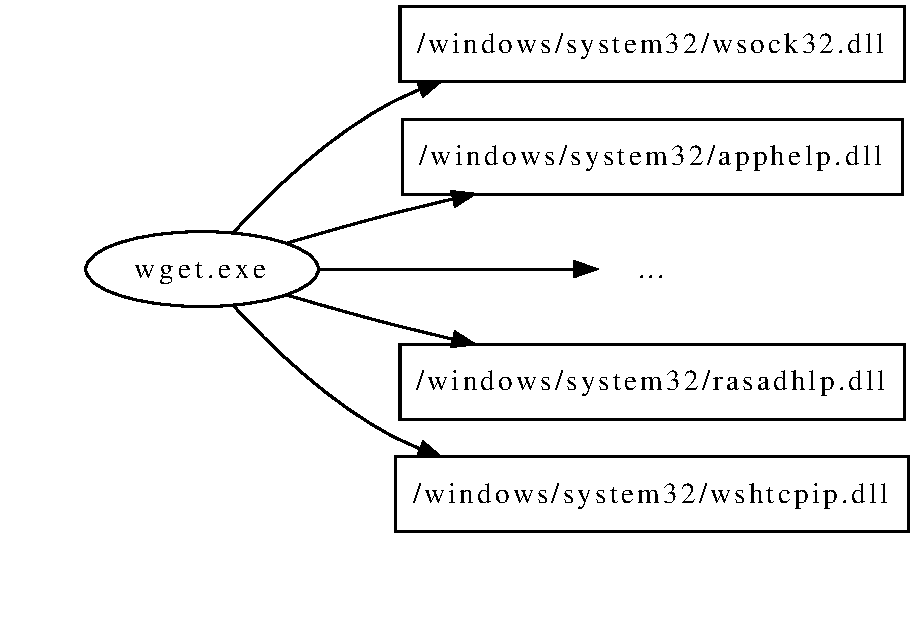
\includegraphics[width=0.5\textwidth]{depvis/wget-exe-split.pdf}
\caption{EXE dependency graph of \code{wget}}
\label{fig:wget-exe-split}
\end{figure}

We illustrate the two dependency graphs on a small example, namely, the
{\tt wget} program downloading an {\tt https} page.
Figure~\ref{fig:wget-exe-split} shows the EXE dependency graph for {\tt wget}.
{\tt wget} loads 34 DLLs,
but the figure only shows 4 of them for simplicity.
The EXE dependency graph is meant for comparing multiple EXE's to show
grouped dependencies.
When there is only a single EXE in the graph, it reduces to a single level
tree.
Figure~\ref{fig:boot}, \ref{fig:browsers} and \ref{fig:depvis-word}
are EXE dependency graphs with multiple EXEs.

\begin{figure}[thb]
\centering
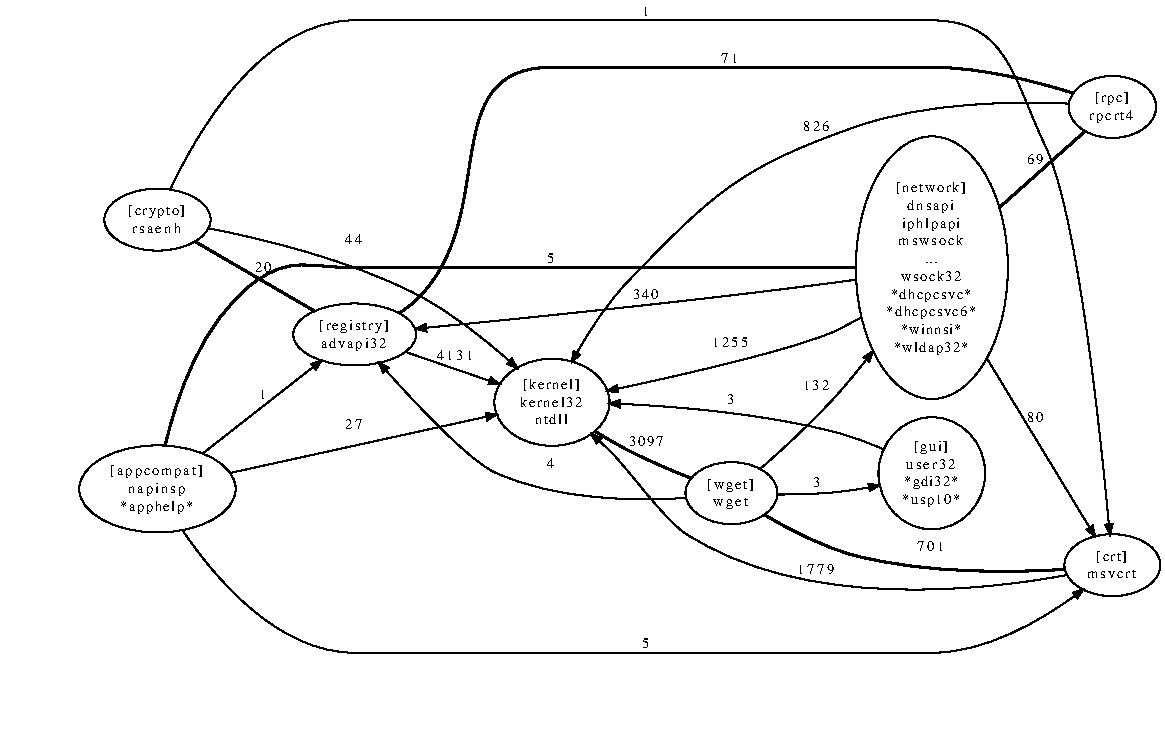
\includegraphics[width=1.0\columnwidth]{depvis/wget-function.pdf}
\caption{DLL dependency graph of {\tt wget} grouped by functionality}
\label{fig:wget-function}
\end{figure}

Figure~\ref{fig:wget-nogroup} shows the DLL
dependency graph for wget without grouping; while
Figure~\ref{fig:wget-function} shows it grouped by functionality.
The edge weights are the number of control transfers between DLLs or EXEs.
As we can see, Figure~\ref{fig:wget-function} is much more compact
because the nodes have been grouped according to the function of the modules.

We manage the assignment of files to groups with a database which is
used by the visualization program.
A table in the database has three fields: binary,
grouping method and group name.
Each binary file is assigned to a group under each grouping method.
For example, the binary {\tt user32.dll} is assigned to the {\tt gui}
functionality group.
As there is no single source of information for all the binaries, we mainly
searched on the Internet for information using the binary's name.
We also used the DLL's exported functions and file version metadata
as heuristics.

For vendor grouping, the assignment of most binaries was done automatically
using the ``Company'' information embedded in the file version metadata.
In some cases, some binaries do not have metadata, so a manual process
was used.
One can also have other and multiple mappings beyond the two which we used.
In this work, we only used a
common mapping for functionality and vendor mappings
in all the dependency graphs.
The grouping process as a whole is relatively static and can mostly be
done once so while some manual effort is needed to create an initial
database, the database may only need to be updated infrequently.

Figure~\ref{fig:wget-nogroup} shows the interactions
between the various DLLs used by {\tt wget}.
It illustrates that a small program already
gives a complex dependency graph.
As such, it may be more useful to check some specific details.
Figure~\ref{fig:wget-function} gives
a ``big picture'' of the dependencies
in {\tt wget} in terms of how the various functional
components interact.
We see that a number of DLLs are loaded but not used in our https download
(files of the form {\it *x*}).

